\documentclass[12pt]{article}
\author{Hugo Thomas}
\usepackage{ amssymb }
\usepackage{ bbm }
\usepackage{ braket }
\usepackage{ mathrsfs }
\usepackage{ geometry }
\usepackage{ amsmath }
\usepackage[alphabetic]{amsrefs}
\usepackage{ hyperref }
\usepackage{braket}
\usepackage{ multicol }
\setlength{\columnsep}{0.8cm}
\usepackage{ sectsty } % section font size
\sectionfont{\fontsize{14}{15}\selectfont}
\subsectionfont{\fontsize{12}{15}\selectfont}
\usepackage{ caption }
\usepackage{ pgfplots }
\pgfplotsset{compat=newest}

\renewcommand{\L}{\mathcal{L}}
\newcommand{\NS}{\mathcal{NS}}
\newcommand{\Q}{\mathcal{Q}}
\newcommand{\tr}[1]{\text{tr}\big[#1\big]}
\newcommand{\note}{\paragraph{Note:}}


\newenvironment{Figure}
  {\par\medskip\noindent\minipage{\linewidth}}
  {\endminipage\par\medskip}


% \usepackage[nottoc, notlof, notlot]{tocbibind}
\geometry{
	a4paper,
 	left=15mm,
 	right=15mm,
 	top=15mm,
	bottom=25mm
}

\makeatletter
\renewcommand{\maketitle}{\bgroup\setlength{\parindent}{0pt}
\begin{flushleft}
  \textbf{\@title}

  \@author
\end{flushleft}\egroup
}
\makeatother

\title{Quantum information project - reading notes}
\begin{document}
\maketitle

\begin{multicols}{2}

\begin{abstract}
	This documents gathers reading notes and solutions found during the project.
\end{abstract}
% \tableofcontents

\vspace{2cm}

% \section*{Bell non locality \cite{2014-bell-nonlocality}}

\section*{Self-testing of quantum systems: a review
\cite{2020-self-testing-a-review}}

\subsection*{The self-testing scenario}

$\mathscr{L(H)}$ denotes the set of linear operators acting on Hilbert space
$\mathscr H$. We know there exist measurement operators $M_{a|x} \in
\mathscr{L(H)}$ acting on Alice's Hilbert space and satisfying

\begin{equation}
	M_{a|x} \succcurlyeq 0 ; \forall a, x \sum_a M_{a|x} = \mathbbm{1}_A
\end{equation}
Similarly, there exist measurement operators $N_{b|y} \in \mathscr{L(H)}$ acting
on Bob's Hilbert space. The measurement operators are therefore projective :
\begin{equation}
	\begin{aligned}
		\forall a, a' & : \quad M_{a|x}M_{a'|x} = \delta_{a, a'}M_{a|x} \\
		\forall b, b' & : \quad N_{b|y}N_{b'|y} = \delta_{b, b'}N_{b|y}
	\end{aligned}
\end{equation}
Now, from the Born rule, there must exist some quantum state $\rho_{AB} \in
\mathscr{L(H_\text{A} \otimes H_\text{B})} \succcurlyeq 0$, and tr$\rho_{AB}$ =
1 such that
\begin{equation}
	p(a,b|x,y) = \tr{\rho_{AB} M_{a|x} \otimes N_{b|y}}
\end{equation}
In self-testing, one aims to infer the form of the state and the measurement in
the trace from knowledge of the correlation $p(a, b|x, y)$ alone, i.e. in
device-independent scenario.
\\\noindent
%% Definition or theorem or smthing
\textbf{Born rule} : A key postulate of quantum mechanics which gives the
probability that a measurement of a quantum system will yield a given result.
More formally, for a state $\ket{\psi}$ and an $F_i$ POVM element (associated
with the measurement outcome $i$), then the probability of obtaining $i$ when
measuring $\ket{\psi}$ is given by

\begin{equation}
	p(i) = \braket{\psi | F_i | \psi}
\end{equation}

\subsection*{Physical assumptions}

\begin{enumerate}
	\item The experiment admits a quantum description (state and measurement)
	\item The laboratories of Alice and Bob are located in separate location in
		space and there is no communication between the two laboratories.
	\item The setting $x$ and $y$ are chosen freely and independently of all
		other systems in the experiment.
	\item Each round of the experiment is independent of all other rounds a
		physically equivalent to all others (i.e. there exists a single density
		matrix and measurement operators that are valid in every round).
\end{enumerate}


\subsection*{Impossibility to infer exactly the references}

\begin{enumerate}
	\item \textit{Unitary invariance of the trace} : one can reproduce the
		statistics of any state $\ket{\psi}$ and measurement $\{M_{a|x}\},
		\{N_{b|y}\}$ by instead using the rotated state $U \otimes V \ket{\psi}$
		and measurement $\{UM_{a|x}U^\dagger\}, \{VN_{b|y}V^\dagger\}$, where
		$U, V$ are unitary transformations. Hence, one can never conclude that
		the state was $\ket{\psi}$ or $U \otimes V \ket{\psi}$. \newline On the
		other hand, considering real reference states $(\ket{\psi} =
		\ket{\psi}^*)$, one can only self-test measurements that are invariant
		under the complex conjugate $*$, since, assuming a real state
		$\ket{\psi}$, $p(ab|xy) = \tr{\ket{\psi}\bra{\psi} M_{a|x}
		\otimes N_{b|y}} = \tr{\ket{\psi}\bra{\psi} M_{a|x}^*
		\otimes N_{b|y}^*}$. Thus, any correlation obtained using
		$\big\{\ket{\psi}, M_{a|x}, N_{b|y} \big\}$ can also be obtained using
		$\big\{\ket{\psi}, M_{a|x}^*, N_{b|y}^* \big\}$; but the second is not
		related to the first one via a local isometry (It's an open problem to
		list the set of state and measurement transformation that do not affect
		the probabilities).

	\item \textit{Additional degrees of freedom} : a state $\ket{\psi} \otimes
		\ket \xi$ and measurements $\{M_{a|x} \otimes \mathbbm{1}_\xi\},
		\{N_{b|y} \otimes \mathbbm{1}_\xi\}$ gives the same correlation as
		$\ket{\psi}$ and $\{M_{a|x}\}, \{N_{b|y}\}$.
\end{enumerate}


\subsection*{Extractability relative to a Bell Inequality}

The extractability $\Xi$ is defined as the maximum fidelity of $\Lambda_A
\otimes \Lambda_B \big[\rho\big]$ and $\ket{\psi'}$ over all CPTP (Completely
positive and trace preserving) maps:
\begin{equation}
	\Xi (\rho \rightarrow \ket{\psi'}) =
	\text{max}_{\Lambda_A ,\Lambda_B} F(\Lambda_A \otimes \Lambda_B, \ket{\psi'})
\end{equation}
where $\rho \rightarrow \ket{\psi'}$ defines a kind of mapping of the test state
$\rho$ to the target state $\ket{\psi'}$. The maximum is taken over all quantum
channels (why are the $\Lambda_{A,B}$ called \textit{quantum channels} ?). This
implies that $\Xi$ return the $\Lambda_{A,B}$ such that the fidelity to the
reference state is maximal.
\\\noindent
In order to test the entanglement characteristics of $\rho$, $\ket{\psi'}$ is
assumed to be a state which achieves the maximal quantum violation. Hence, when
the maximal quantum violation is observed in a self-testing scenario, the shared
unknown state $(\rho)$ can be mapped to $\ket{\psi'}$, and the resulting
extractability is 1.
\\\noindent
To get the optimal (robustness-wise) self-testing statement, one can minimize
the possible extractability (over all states) when a violation of at least
$\beta$ is observed on a Bell inequality $B$. This quantity can be captured by
the function $\Q$ defined as

\begin{equation}
	\Q_{\psi,\mathcal{B}_\mathcal{I}} = \text{min}_{\rho \in
	S_\mathcal{B}(\beta)} \quad \Xi (\rho \rightarrow \ket{\psi'})
\end{equation}
where $S_\mathcal{B}(\beta)$ is the set of states $\rho$ which violate Bell
inequality $\mathcal B$ as defined in
\cite{2018-experimentally-robust-self-testing} with value at least $\beta$.  One
needs to note that the optimal CPTP map generally depends on the observed
violation.

\section*{The device-independent outlook on quantum physics
\cite{scarani2015deviceindependent}}

\subsection*{Formal characterization of local variables}

The local variable paradigm is related to the idea of pre-established agreement
between the two parties, i.e. the output of each run is fully determined by a
variable $\lambda$:
\begin{equation}
	\mathbb{P}(a,b|x,y, \lambda) =
		\mathbb{P}(a|x, \lambda) \mathbb{P}(b|y, \lambda)
\end{equation}
In other words, one can write the probability of having ($a$, $b$) given the two
inputs ($x$, $y$) as:
\begin{equation}
	\mathbb{P}(a, b|x, y) =
		\int d\lambda\mathbb{P}(a|x, \lambda) \mathbb{P}(b|y, \lambda)
\end{equation}
This pre-established agreement is called \textit{shared randomness}.
\\\noindent
\textit{No-signalling condition} : The fact that the statistics of $a$ ($b$)
should nod depend on $y$($x$), that is, the following conditions hold for all
$a, b, x, y, \lambda$:
\begin{equation}
	\mathbb{P}(a|x, y, \lambda) = \mathbb{P}(a|x, \lambda)
	\qquad
	\mathbb{P}(b|x, y, \lambda) = \mathbb{P}(b|y, \lambda)
\end{equation}
\\\noindent
From the above conditions one can deduce the \textit{no-signalling constraints} :
\begin{equation}
	\begin{aligned}
		\forall x, x' \in \mathcal{Y}: &
			\sum_b \mathbb{P}(a,b|x,y) =
			\sum_b \mathbb{P}(a,b|x,y') = \mathbb{P}(a|x) \\
		\forall x, x' \in \mathcal{X}: &
			\sum_a \mathbb{P}(a,b|x,y) =
			\sum_a \mathbb{P}(a,b|x',y) = \mathbb{P}(b|y) \\
	\end{aligned}
\end{equation}

\subsection*{Bell inequalities as a polytope}
The set $\L$ of all families of probability distributions that can be obtained
with LV is convex. In other words, if $\mathcal P_1 \in \L$ and $\mathcal P_2
\in \L$, then $\forall \alpha \in [0, 1] : \alpha \mathcal P_1 + (1-\alpha)
\mathcal P_2 \in \L $. Furthermore, each deterministic local point is an
extremal point of $\L$. \\\noindent A polytope $\L$ in $\mathbb R^d$ is
delimited by finitely many ($d-1$)-dimensional hyperplanes called facets (of the
polytope).

% \subsubsection*{Minimal $d$ such that $\L \in \mathbbm{R}^d$}

\section*{Link between Bell inequalities and linear programming}
It is possible to state to which set $( \L, \Q, \NS )$ a probability distribution $P$ belongs to.
Consider the linear program given below:
\begin{equation} \label{eq:primal}
	\begin{aligned}
			 & \min \quad q \\
		s.t. &
		\begin{cases}
			(1-q) P + q \mathbbm{1}  & = \sum_\lambda \mu_\lambda D_\lambda \\
			\sum_\lambda \mu_\lambda & = 1 \\
			q & \leq 1 \\
			\forall \lambda, \mu_\lambda \geq 0, q \geq 0
		\end{cases}
	\end{aligned}
\end{equation}
where $\{D_\lambda\}_\lambda$ is the set of all deterministic behaviors as
described in \cite{2014-bell-nonlocality} and $\mathbbm{1}$ is the vector
$\begin{pmatrix} 0.5 \cdots 0.5 \end{pmatrix}^T$ that represents a fully random
noise. If the result is $q = 0$, then the probability vector $P$ describes a
local model, otherwise, if $q > 0$, the probability vector describes a quantum
behavior.

The dual program of the program (\ref{eq:primal}) is the following:

\begin{equation} \label{eq:dual}
	\begin{aligned}
 			 & \max \quad -\Gamma \cdot P + \phi - \omega \\
		s.t. &
		\begin{cases}
			- \Gamma \cdot D_\lambda + \phi & \leq 0, \forall \lambda \in \big\{1, \cdots, \Delta^{2m}\big\} \\
			\Gamma \cdot (\mathbbm{1} - P) - \omega & \leq 1 \\
			\forall \lambda, \gamma_\lambda \in \mathbb{R}, \quad \omega \geq 0,  & \phi \in \mathbb{R}
		\end{cases}
	\end{aligned}
\end{equation}
where $\Gamma = \begin{pmatrix} \gamma_1 \cdots \gamma_{\Delta^{2m}}
\end{pmatrix}^T$. We need to discuss the above program.

\subsection*{Non-linear programming to determine a probability vector}
Considering the linear program (\ref{eq:primal}), one can transform the vector $P$
into a vector of variables. Adding the constraints for $P$ to be a probability
vector, one can solve the associated non-linear program. It yields the following
non-linear program
\begin{equation} \label{eq:primal-nl}
	\begin{aligned}
			  & \max \quad CHSH\\
		s.t.  &
		\begin{cases}
			(1-q) P + q \mathbbm{1}  & = \sum_\lambda \mu_\lambda D_\lambda \\
			\sum_\lambda \mu_\lambda & = 1 \\
			q & \leq 1 \\
			\forall \lambda, \mu_\lambda \geq 0, q \geq 0
		\end{cases}
	\end{aligned}
\end{equation}
where $CHSH$ is the CHSH inequality:
\begin{equation}
	\braket{A_0 \otimes B_0} +
	\braket{A_1 \otimes B_0} +
	\braket{A_0 \otimes B_1} -
	\braket{A_1 \otimes B_1}
\end{equation}
and expectation value can be decomposed in terms of measurement operators such that:
\begin{equation}
	\braket{A_x \otimes B_y} = \braket{(M_{1|x} - M_{-1|x})\otimes(M_{1|y} - M_{-1|y})}
\end{equation}
and considering
\begin{equation}
	p(ab|xy) = \braket{M_{a|x} \otimes M_{b|y}}
\end{equation}
where each $p(ab|xy)$ becomes a variable.

This can be resolved by Gurobi Solver \cite{gurobi} even though the program
found is non-convex.

\note It should be possible to add a constraint to ensure the resulting
probability vector $P$ stays in $\Q$ to get the maximal violation of the CHSH
inequality. Otherwise, the maximal value is $4$ meaning that the probability
vector is in $\NS$. Considering the additional constraint $CHSH \leq 2 \sqrt 2$
(that ensure that $P$ is \textit{at most} in $\Q$), we obtain in $P$ the
probabilities that maximally violate the CHSH inequality, and $q = 0.91$ which
is consistent with what we could expect considering the program
(\ref{eq:primal}).

\subsection*{Considering a noisy channel}

\begin{Figure}
% This file was created with tikzplotlib v0.10.1.
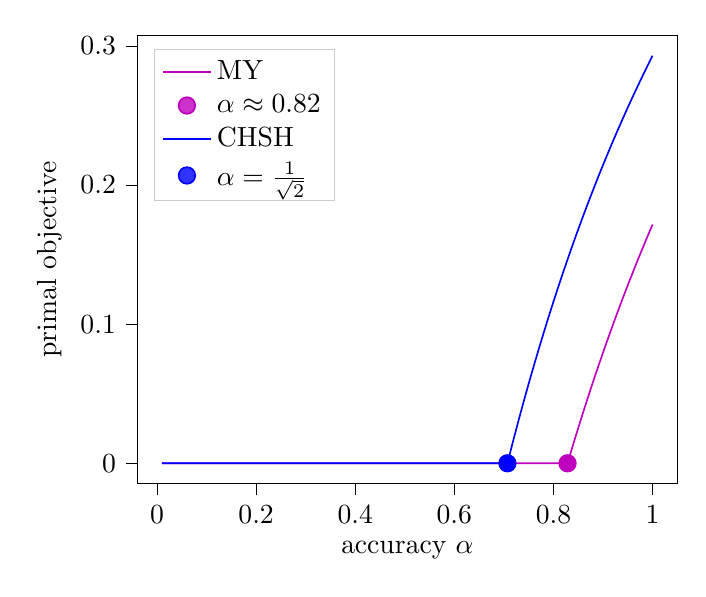
\begin{tikzpicture}

\definecolor{darkgray176}{RGB}{176,176,176}
\definecolor{darkviolet1910191}{RGB}{191,0,191}
\definecolor{lightgray204}{RGB}{204,204,204}

\begin{axis}[
legend cell align={left},
legend style={
  fill opacity=0.8,
  draw opacity=1,
  text opacity=1,
  at={(0.03,0.97)},
  anchor=north west,
  draw=lightgray204
},
tick align=outside,
tick pos=left,
x grid style={darkgray176},
xlabel={accuracy \(\displaystyle \alpha\)},
xmin=-0.0395000000000008, xmax=1.0495,
xtick style={color=black},
y grid style={darkgray176},
ylabel={primal objective},
ymin=-0.0146446609406726, ymax=0.307537879754125,
ytick style={color=black}
]
\addplot [semithick, darkviolet1910191]
table {%
1 0.17157287525381
0.99 0.163204924498798
0.98 0.154666199238581
0.97 0.145951417787433
0.96 0.137055078389385
0.95 0.127971447635589
0.94 0.118694548142351
0.93 0.109218145434204
0.92 0.0995357339715324
0.91 0.0896405222569338
0.9 0.0795254169486775
0.89 0.069183005903157
0.88 0.0586055400611474
0.87 0.0477849140848387
0.86 0.0367126456439648
0.85 0.0253798532397762
0.84 0.0137772324450116
0.83 0.00189503042627678
0.82 0
0.81 0
0.8 0
0.79 0
0.78 0
0.77 0
0.76 0
0.75 0
0.74 0
0.73 0
0.72 0
0.71 0
0.7 0
0.69 0
0.68 0
0.67 0
0.66 0
0.65 0
0.64 0
0.63 0
0.62 0
0.61 0
0.6 0
0.59 0
0.58 0
0.57 0
0.56 0
0.55 0
0.54 0
0.53 0
0.52 0
0.51 0
0.5 0
0.49 0
0.48 0
0.47 0
0.46 0
0.45 0
0.44 0
0.429999999999999 0
0.419999999999999 0
0.409999999999999 0
0.399999999999999 0
0.389999999999999 0
0.379999999999999 0
0.369999999999999 0
0.359999999999999 0
0.349999999999999 0
0.339999999999999 0
0.329999999999999 0
0.319999999999999 0
0.309999999999999 0
0.299999999999999 0
0.289999999999999 0
0.279999999999999 0
0.269999999999999 0
0.259999999999999 0
0.249999999999999 0
0.239999999999999 0
0.229999999999999 0
0.219999999999999 0
0.209999999999999 0
0.199999999999999 0
0.189999999999999 0
0.179999999999999 0
0.169999999999999 0
0.159999999999999 0
0.149999999999999 0
0.139999999999999 0
0.129999999999999 0
0.119999999999999 0
0.109999999999999 0
0.0999999999999992 0
0.0899999999999992 0
0.0799999999999993 0
0.0699999999999993 0
0.0599999999999993 0
0.0499999999999993 0
0.0399999999999993 0
0.0299999999999992 0
0.0199999999999992 0
0.00999999999999925 0
};
\addlegendentry{MY}
\addplot [semithick, darkviolet1910191, mark=*, mark size=3, mark options={solid}, only marks]
table {%
0.828428781600444 0
};
\addlegendentry{$\alpha \approx 0.82$}
\addplot [semithick, blue]
table {%
1 0.292893218813452
0.99 0.285750726074194
0.98 0.278462468176992
0.97 0.271023936921085
0.96 0.263430436264013
0.95 0.255677072435213
0.94 0.247758743418566
0.93 0.2396701277564
0.92 0.231405672623318
0.91 0.222959581113684
0.9 0.214325798681614
0.89 0.2054979986668
0.88 0.196469566833469
0.87 0.187233584843049
0.86 0.177782812573782
0.85 0.168109669192297
0.84 0.158206212873158
0.83 0.148064119052352
0.82 0.137674657089576
0.81 0.127028665201793
0.8 0.116116523516815
0.79 0.104928125080319
0.78 0.093452844632631
0.77 0.0816795049525354
0.76 0.0695963405440161
0.75 0.0571909584179363
0.74 0.0444502956938543
0.73 0.0313605737170578
0.72 0.0179072483520168
0.71 0.00407495607528462
0.7 0
0.69 0
0.68 0
0.67 0
0.66 0
0.65 0
0.64 0
0.63 0
0.62 0
0.61 0
0.6 0
0.59 0
0.58 0
0.57 0
0.56 0
0.55 0
0.54 0
0.53 0
0.52 0
0.51 0
0.5 0
0.49 0
0.48 0
0.47 0
0.46 0
0.45 0
0.44 0
0.429999999999999 0
0.419999999999999 0
0.409999999999999 0
0.399999999999999 0
0.389999999999999 0
0.379999999999999 0
0.369999999999999 0
0.359999999999999 0
0.349999999999999 0
0.339999999999999 0
0.329999999999999 0
0.319999999999999 0
0.309999999999999 0
0.299999999999999 0
0.289999999999999 0
0.279999999999999 0
0.269999999999999 0
0.259999999999999 0
0.249999999999999 0
0.239999999999999 0
0.229999999999999 0
0.219999999999999 0
0.209999999999999 0
0.199999999999999 0
0.189999999999999 0
0.179999999999999 0
0.169999999999999 0
0.159999999999999 0
0.149999999999999 0
0.139999999999999 0
0.129999999999999 0
0.119999999999999 0
0.109999999999999 0
0.0999999999999992 0
0.0899999999999992 0
0.0799999999999993 0
0.0699999999999993 0
0.0599999999999993 0
0.0499999999999993 0
0.0399999999999993 0
0.0299999999999992 0
0.0199999999999992 0
0.00999999999999925 0
};
\addlegendentry{CHSH}
\addplot [semithick, blue, mark=*, mark size=3, mark options={solid}, only marks]
table {%
0.707108195400103 0
};
\addlegendentry{$\alpha = \frac{1}{\sqrt{2}}$}
\end{axis}

\end{tikzpicture}

\captionof{figure}{Noise resistance of each probability distributions}
\end{Figure}

\end{multicols}

\bibliographystyle{alpha}
\bibliography{bibliography}
\end{document}